\section{Optical Dipole Trapping}

The use of \glspl{odt} in the cold-atom electron source will allow greater stability of the atom cloud during ionisation and extraction as well as increasing the density of the atom cloud during these phases.

\subsection{History of optical dipole trapping}
The use of the optical dipole force as a confining mechanism was first proposed by Askar'yan in 1962\cite{askaryan_effects_1962} for plasmas and neutral atoms. Ashkin successfully demonstrated the trapping of micron-size latex spheres suspended in water using a focused Gaussian lasers in 1970\cite{ashkin_acceleration_1970}. The first optical trapping of atoms was demonstrated by Chu et. al. in 1986\cite{chu_experimental_1986} where a \gls{odt} was used to trap sodium atoms.

Since then \glspl{odt} have been used extensively in atom optics especially in the creation of \glspl{bec} and atom lasers.

\subsection{Theory of Dipole Trapping}
\Glspl{odt} are sometimes considered to be the simplest form of atom trap for two-level atoms since they consist solely of a focused, Gaussian laser beam detuned from the atomic resonances. The intensity of the Gaussian laser beam at the beam waist varies transversely with $r$ as
\begin{equation}
I(r) = I_0e^{-r^2 / w_0^2},
\end{equation}
where $I_0$ is the intensity at the centre of the beam at the waist, $r$ is the radial distance from the centre of beam and $w_0$ is the beam radius at the focus.

The ground state light shift for ground state atoms in the laser field is given by\cite{metcalf_laser_1999}
\begin{equation}
\Delta E_g = \frac{\hbar \Omega^2}{4\delta},
\end{equation}
where the Rabi frequency $\Omega^2= \gamma^2 I / 2 I_s$ and $\gamma$ is the linewidth, $I$ is the light intensity and $I_s$ is the saturation intensity. Thus the light shift is larger at points of high intensity such as the centre of the beam and the beam focus.

In order to trap the laser is detuned below the resonances such that $\delta = \omega_l - \omega_a < 0$ where $\omega_l$ is the laser frequency and $\omega_a$ is the atomic resonance frequency. With negative detuning the ground-state light shift is negative everywhere and thus atoms feels a force towards the centre given by the gradient of the light shift, and for $\delta \gg \Omega$ and $\delta \gg \gamma$ the force is given by
\begin{equation}
F \simeq - \frac{\hbar}{4\delta} \nabla(\Omega(r)^2) = -\frac{\hbar \gamma^2}{8\delta I_s} \nabla I (r).
\end{equation}

At the focus of a Gaussian beam this force is
\begin{equation}
F \simeq \frac{\hbar \gamma^2}{4 \delta} \frac{I_0}{I_s} \frac{r}{w_0^2} e^{-r^2/w_0^2},
\end{equation}
and thus the transverse trapping potential is given by
\begin{equation}
U = -\int dr F \simeq \frac{\hbar \gamma^2}{8\delta} \frac{I_0}{I_s} e^{-r^2/w_0^2}.
\end{equation}

It is easy to see with this equation how a negative (red) detuning will result in an inwards, trapping force and a positive (blue) detuning will result in a outwards, repulsive force. Blue detuned lasers can be used for trapping if the beam has a low intensity centre however\cite{davidson_long_1995, lee_raman_1996, ozeri_long_1999, friedman_compression_2000}.

\subsubsection{Scattering rates}
Atoms in near-resonant light fields experience a non-conservative force due to excitation and spontaneous decay (ie. scattering). More general expressions for the trapping potential can be used to compare the trap potential to the scattering rate due to the photon absorption\cite{grimm_optical_2000}
\begin{equation}
U_{dip}(\vec{r})=\frac{3\pi c^2}{2\omega_0^3} \frac{\gamma}{\delta} I(\vec{r})
\end{equation}
\begin{equation}
\Gamma_{sc}(\vec{r})=\frac{3\pi c^2}{2\hbar \omega_0^3}\left(\frac{\gamma}{\delta}\right)^2 I(\vec{r})
\end{equation}

The scattering rate should be kept to a minimum in order to prevent the heating atoms in the trap. Fortunately the relationships are such that for large detunings $U_{dip}\gg\Gamma_{sc}$. Such far detuned lasers however do create shallower traps and thus require more powerful lasers to create similar trap depths.

\subsection{Using an optical dipole trap in a cold-atom electron source}
An \gls{odt} can serve several purposes in the cold-atom electron source including increasing the brightness and coherence of the electron bunches as described earlier.

A number of design choices in the development of this dipole trap are under consideration such as the wavelength of the trap, the configuration of the trapping beam/s and the size of the beam waist.

\subsubsection{Available equipment}
Two main options are available as far as light sources for the trap,
\begin{itemize}
    \item a 20mW, 780nm diode laser amplified by a \gls{ta} to 1.8W,
    \item a 20W, 1064nm fibre laser.
\end{itemize}

The 780nm diode laser that seeds the \gls{ta} can be tuned away from the 780nm resonance by tens of nanometres however the \gls{ta} has a maximum wavelength of 785nm. This restricts the possible red detuning to a maximum of 5nm.

The 1064nm laser is extremely far away from the resonances which results in reduced scattering rates however lasers with powers as high as 20W require more caution in their use as well as suitable optics capable of dealing with the high-intensity light.

\subsubsection{1064nm optical dipole traps}
\Glspl{odt} with a wavelength near 1064nm are frequently used when rubidium \glspl{bec} are being formed \cite{chikkatur_continuous_2002, couvert_quasi-monomode_2008, kleine_buning_slow_2010, lin_rapid_2009, arnold_all-optical_2011, fu_bose-einstein_2011}. These \glspl{bec} are used for many different applications including the creation of atom-lasers \cite{kleine_buning_slow_2010, chikkatur_continuous_2002, couvert_quasi-monomode_2008}, atomic clocks\cite{kleine_buning_extended_2011} and obviously further studies into \glspl{bec} themselves and related trapping mechanisms \cite{arnold_all-optical_2011, fu_bose-einstein_2011, lin_rapid_2009}.

\glspl{odt} with wavelengths at 1064nm are not only used in rubidium \glspl{bec}. They have to used to form \glspl{bec} of caesium\cite{hung_accelerating_2008}, chromium\cite{beaufils_all-optical_2008}, double-species \glspl{bec}\cite{thalhammer_double_2008}, and even molecular \glspl{bec}\cite{zwierlein_observation_2003}.

\subsubsection{``Near" 780nm optical dipole traps}
Traps made from lasers ``near'' 780nm are more often used when studying and developing trapping methods. Such traps have detunings that vary from 0.5nm\cite{miller_rf-induced_2002} to over 60nm\cite{miller_far-off-resonance_1993, weber_analysis_2006} and are usually referred to as \glspl{fort}. Some of the things that these laser have been used to study are dipole trap loading\cite{kuppens_loading_2000}, trapping single atoms\cite{weber_analysis_2006} and the combination of an \gls{odt} with Sisyphus cooling\cite{miller_rf-induced_2002}.

\subsubsection{Configurations}
The simplest \gls{odt} consists simply of a focused Gaussian beam\cite{chu_experimental_1986} and many of the references use this simple configuration.

\begin{figure}[h]
	\centering
	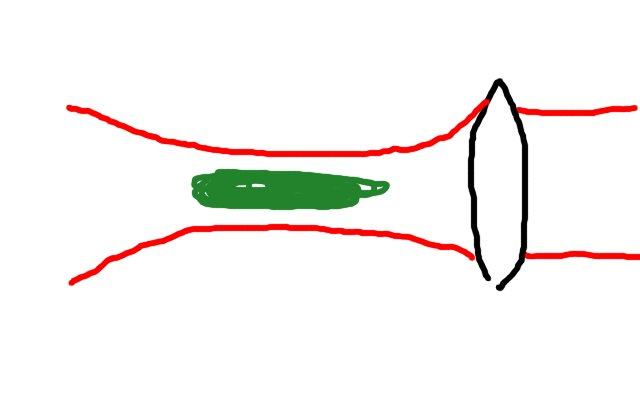
\includegraphics[scale=0.32]{figs/simpledipoletrap.jpg}
	\caption[Title]{A simple \gls{odt} configuration}
	\label{figs/MOT.pdf}
\end{figure}

Crossed dipole traps\cite{barrett_all-optical_2001, xiong_evaporative_2010, arnold_all-optical_2011, fu_bose-einstein_2011} are a more complicated configuration that can provide a stronger trap as well as control over the shape of the trap and the trapping potentials in various directions. Unlike simple dipole traps which create long cigar-shaped traps crossed dipole traps can create spherical traps.

\begin{figure}[h]
	\centering
	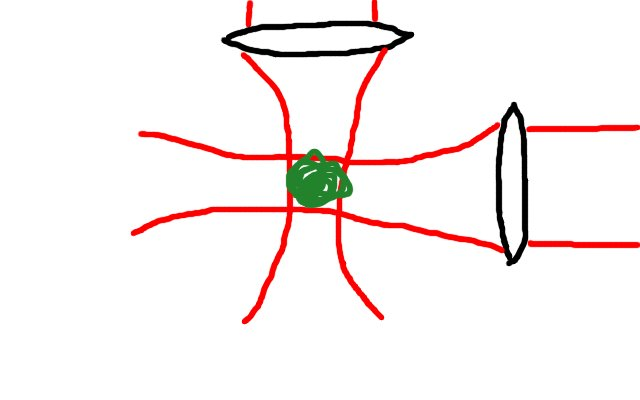
\includegraphics[scale=0.32]{figs/crosseddipoletrap.jpg}
	\caption[Title]{A crossed \gls{odt} configuration}
	\label{figs/MOT.pdf}
\end{figure}

Crossed dipole traps do not require the beams to be at right angles. For example Couvert et. al. \cite{couvert_quasi-monomode_2008} have their beams at 45 degrees when generating atom lasers.

Kinoshita et. al.\cite{kinoshita_all-optical_2005} use a crossed dipole configuration where the two beams do not cross at their respective foci. Instead the beams are crossed at the desired beam waist (initially $\mathrm{300\mu m}$ in this case) after which the waists at the trapping point can be dynamically controlled by adjusting the positions of the lens.


\subsubsection{Waist size}
The size of the beam waist is an important factor for the performance of \glspl{odt}. In most experiments involving dipole traps the beam waist used is in the region of $\mathrm{30\mu m}$ in order to provide the deepest trap possible. For the cold-atom electron source however it may be desirable to use a broader trap in order to trap a larger number of atoms. Then again the deepest trap attainable may provide better results.

In order to provide an easily modifiable beam waist a setup like the one describe in figure \ref{figs/MOT.pdf} which consists of a beam expander consisting of a concave then convex lens followed by the focusing lens could be used.

\begin{figure}[h]
	\centering
	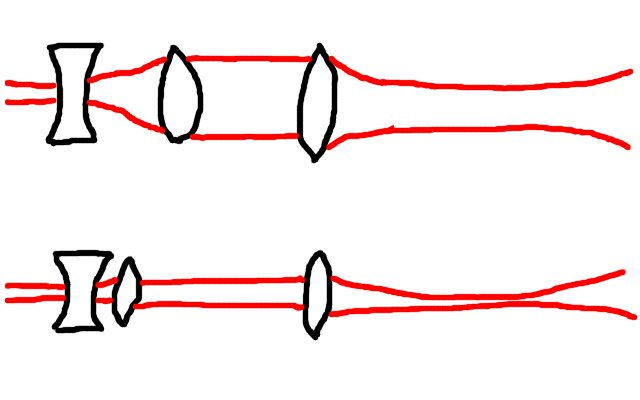
\includegraphics[scale=0.32]{figs/waistcontrol.jpg}
	\caption[Title]{An example setup for controlling the beam waist}
	\label{figs/MOT.pdf}
\end{figure}

This configuration allows manipulation of the size of the beam incident on the final lens by adjusting the distance between the lens in the beam expander. This in turn changes the beam waist at the focus according to
\begin{equation}
2w_0=\frac{4\lambda}{\pi}\frac{f}{d}
\end{equation}
where $w_0$ is the beam radius at the focus, $\lambda$ is the wavelength of the light, $f$ is the focal length of the final lens and $d$ is the diameter illuminated by the beam incident on the final lens.


